\documentclass[final]{beamer}

% ====================
% Packages
% ====================

\usepackage[T1]{fontenc}
\usepackage{lmodern}
\usepackage[size=a2,scale=1.0]{beamerposter}
\usetheme{gemini}
\usecolortheme{gemini}
\usepackage{graphicx}
\usepackage{booktabs}
\usepackage{tikz}
\usepackage{pgfplots}
\pgfplotsset{compat=1.14}
\usepackage{anyfontsize}
\usepackage{wrapfig}


% ====================
% Lengths
% ====================

% If you have N columns, choose \sepwidth and \colwidth such that
% (N+1)*\sepwidth + N*\colwidth = \paperwidth
\newlength{\sepwidth}
\newlength{\colwidth}
\setlength{\sepwidth}{0.025\paperwidth}
\setlength{\colwidth}{0.3\paperwidth}
\newcounter{row}
\newcounter{col}
\newcounter{rowa}
\newcounter{cola}


\newcommand{\separatorcolumn}{\begin{column}{\sepwidth}\end{column}}

% ====================
% Title
% ====================

\title{Sudoku is Hard}

\author{Eve Routledge}

%\institute[shortinst]{Durham University}

% ====================
% Footer (optional)
% ====================

\footercontent{
  \href{https://www.example.com}{https://www.example.com} \hfill
  \href{mailto:alyssa.p.hacker@example.com}{eve.routledge@durham.ac.uk}}
% (can be left out to remove footer)

% ====================
% Logo (optional)
% ====================

% use this to include logos on the left and/or right side of the header:
\logoleft{
\includegraphics[height=3cm]{DurhamUniversityLogo_WHITE.png}}

% ====================
% Sudoku
% ====================
\newcommand\setrow[9]{
  \setcounter{col}{1}
  \foreach \n in {#1, #2, #3, #4, #5, #6, #7, #8, #9} {
    \edef\x{\value{col} - 0.5}
    \edef\y{9.5 - \value{row}}
    \node[anchor=center] at (\x, \y) {\n};
    \stepcounter{col}
  }
  \stepcounter{row}
}

\newcommand\setrowa[3]{
  \setcounter{cola}{1}
  \foreach \n in {#1, #2, #3} {
    \edef\x{\value{cola} - 0.5}
    \edef\y{3.5 - \value{rowa}}
    \node[anchor=center] at (\x, \y) {\n};
    \stepcounter{cola}
  }
  \stepcounter{rowa}
}
% ====================
% Body
% ====================

\begin{document}

\begin{frame}[t]
\begin{columns}[t]
\separatorcolumn

\begin{column}{\colwidth}
  \begin{exampleblock}{Sudoku: An Introduction}

Imagine a sudoku of size $D^2\times D^2$. How big does $D$ have to be for you to need more than a day to solve it? Maybe 6 or 10 or even just 4. Don't worry if you said a smaller number than your friends, this has nothing to do with your problem solving skills, even a computer finds sudoku hard. In fact just incrementing $D$ by 1 leads to an exponential increase in compute time and the most optimal algorithms for solving sudoku are infeasible for $100 \times 100$.

Don't just take my word on it, instead follow this proof as we transform sudoku into a known 'difficult' problem (SAT) that has plagued computer scientists for decades. 

We will transform sudoku to SAT in 4 steps:

   \textbf{Sudoku $\geq_p$ Latin Square $\geq_p$ Triangulate a Tripartite Graph $\geq_p$ 3-SAT $\geq_p$ SAT}.

	\textbf{Def$^\text{n}$}: A valid \textbf{Sudoku} puzzle is a function $ S: i,j \rightarrow x$ for values $i,j \in \{1,...,D^2\}$ and $x \in \{0,...,D^2\}$ satisfying the following:
\begin{itemize}
	\item{for all $a,b,c$  $\in \{1,...,D^2\}$ with $S(a,b)\neq 0$ and $S(a,c)\neq 0$, then $ S(a,b)\neq$ S(a,c) }
	\item{for all $a,b,c$  $\in \{1,...,D^2\}$ with $S(a,b)\neq 0$ and$ S(c,b)\neq 0$, then $S(a,b)\neq$ S(c,b) }
	\item{for all $ a,b,c,d $ $\in \{1,...,D^2\}$ with $a\text{ mod }D = c\text{ mod }D$, $b\text{ mod }D  =  d\text{ mod }D$, $S(a,b)\neq 0$  and $S(c,d) \neq 0$, then $S(a,b)\neq S(a,c)$ }
\end{itemize}
It is completed if $x \in \{1,...,D\}$.


\textbf{Def$^\text{n}$}: A valid \textbf{Latin Square} puzzle is a function $L:i,j \rightarrow x$ for values $i,j \in \{1,..,D\} $ and $x \in \{0,...,D\}$ satisfying the following:
\begin{itemize}
\item{for all $a,b,c \in \{1,...,D\}$ with $L(a,b) \neq 0 $ and $L(a,c) \neq 0$ then $L(a,b) \neq L(a,c)$}
\item{for all $a,b,c \in \{1,...,D\}$ with $L(a,b) \neq 0 $ and $L(c,b) \neq 0$ then $L(a,b) \neq L(c,b)$}
\end{itemize}
It is complete or solved if for all $i,j \in \{1,...,D\}$, $L(i,j) \neq 0$.

\textbf{Def$^\text{n}$}: A graph $G=(V,E)$ is \textbf{Tripartite} if a partition $V_1$, $V_2$, $V_3$ exists such that the vertices are split into three sets with no edges between vertices that belong to the same set, i.e for all $(v_i,v_j) \in E\text{ if } v_i \in V_i\text{ then }v_j \not\in V_i $. A \textbf{Triangulation} T of a graph G is a way to divide all edges into disjoint subsets $T_i$, each forming a triangle ($T_i=\{(v_{1}, v_{2}),(v_{2}, v_{3}),(v_{3},v_{1})\}$).

\textbf{Def$^\text{n}$:} A \textbf{boolean expression} is a formula made of variables $\in B$ and operations (conjunction $\land$, disjunction $\lor$, not $\neg$).A literal is $b\in B$ or $\neg b$. A clause $c\in C$ is a disjunction of literals, $b_1 \lor b_2 \lor ... b_i$. For this to be in conjugate normal form the formula must be a conjunction of clauses. A boolean expression is satisfiable if a truth assignment to all members of $B$ exists such that the expression evaluates to true. 

\textbf{Def$^\text{n}$:}  \textbf{SAT} is the decision problem determining whether a boolean expression is satisfiable or not. \textbf{3-SAT} is an enforced limitation of SAT such that each clause is made up of 3 literals. 
  \end{exampleblock}
 \begin{block}{Computational Complexity}

For those with a mathematical mind, outraged by the lack of definitions of 'difficulty' and 'hardness', let's take a detour into complexity theory. 

\textbf{Def$^\text{n}$:} Let $f$ be a function indicating the execution time for an algorithm and $g$ a strictly positive function. $f(x)=O (g(x))$ if $\exists$ positive $ M$ and $x_0$ such that $|f(x)|\leq Mg(x)$ $\forall$ $x\geq x_0$.

\textbf{Def$^\text{n}$:} A \textbf{Reduction}, $A \geq_p B$, is a transformation in $O(x^c)$ from problem $B$ to $A$.

\textbf{Def$^\text{n}$:} A \textbf{Turing Machine} is the mathematical model of a CPU.

 \begin{itemize}
	\item{P is the set of problems solved in polynomial time $O(x^c)$ by a Turing machine;} 
	\item{NP is the set verified in $O(x^c)$ and but not solved in $O(x^c)$ ;} 
	\item{the NP-complete set has problems that any NP problem can be reduced to in $O(x^c)$.} 
\end{itemize}
Problems in P are considered feasible and those in NP are infeasible as their complexity scales exponentially with respect to the input size. This is if we assume $P\neq NP$ which is of course yet to be proven and remains one of the unsolved Millennium Prize problems. 

So when we state sudoku is hard we are actually saying sudoku belongs to NP.

By outlining a reduction Sudoku$ \geq_p $SAT we show sudoku is NP-complete and therfore in NP. 

\textbf{Intuition:} Assume we have an algorithm $\Phi$ solving sudoku in $O(x^{c_1})$ then if there exists a reduction algorithm $\Gamma$ of Sudoku$ \geq_p $SAT in $O(x^{c_2})$  then for a given SAT problem $x$, $\Phi(\Gamma(x))$ will give an algorithm solving SAT in $O(x^{c_1+c_2})$ which, given the Cook-Levin theorem, is a contradiction. 

  \end{block}
  \begin{alertblock}{Cook Levin Theorem}
SAT is NP-complete.
  \end{alertblock}
\end{column}

\separatorcolumn

\begin{column}{\colwidth}
  \begin{block}{SAT $\leq_p$ 3 SAT}
To begin we look at the bread and butter of complexity theory.

Given a SAT instance with the input sets of $B$ and $C$. For each $c \in C$ with more than 3 literals we can transform these to a new set of clauses of length 3. 

For $c = b_1 \lor b_2 \lor ... \lor b_n$ we introduce a new literal: $a_1$ to give $b_1 \lor b_2 \lor a_1$, $\bar{b_1} \lor a_1$, $\bar{b_2} \lor a_1$ and $a_1 \lor b_3 \lor ... \lor b_n$. Then $a_1 \lor b_3 \lor ... \lor b_n$ becomes $b_3 \lor b_4 \lor a_2$, $\bar{b_3} \lor a_2$, $\bar{b_4} \lor a_2$ and $a_1 \lor a_2 \lor b_5 \lor ... \lor b_n$. This continues at most $n/2$ times to give $a_1 \lor ... \lor a_{n/2}$ or $a_1 \lor ... \lor a_{n/2} \lor b_n$ if n is odd. 

Because we can convert a clause larger than 3 into multiple clauses of at most 3 literals in linear time ($O(n/2 + n/4 + ...) = O(n)$) this means we can reduce SAT to 3SAT in polynomial time. 

3SAT is NP-Complete. $\square$

  \end{block}
  \begin{block}{Triangulated Tripartite Graph $\geq_p$ 3 SAT}
This reduction is a little trickier as we need to introduce the Holyer graph $H$ which dips a toe into topology as it is a torus.

\begin{wrapfigure}{r}{7cm}
		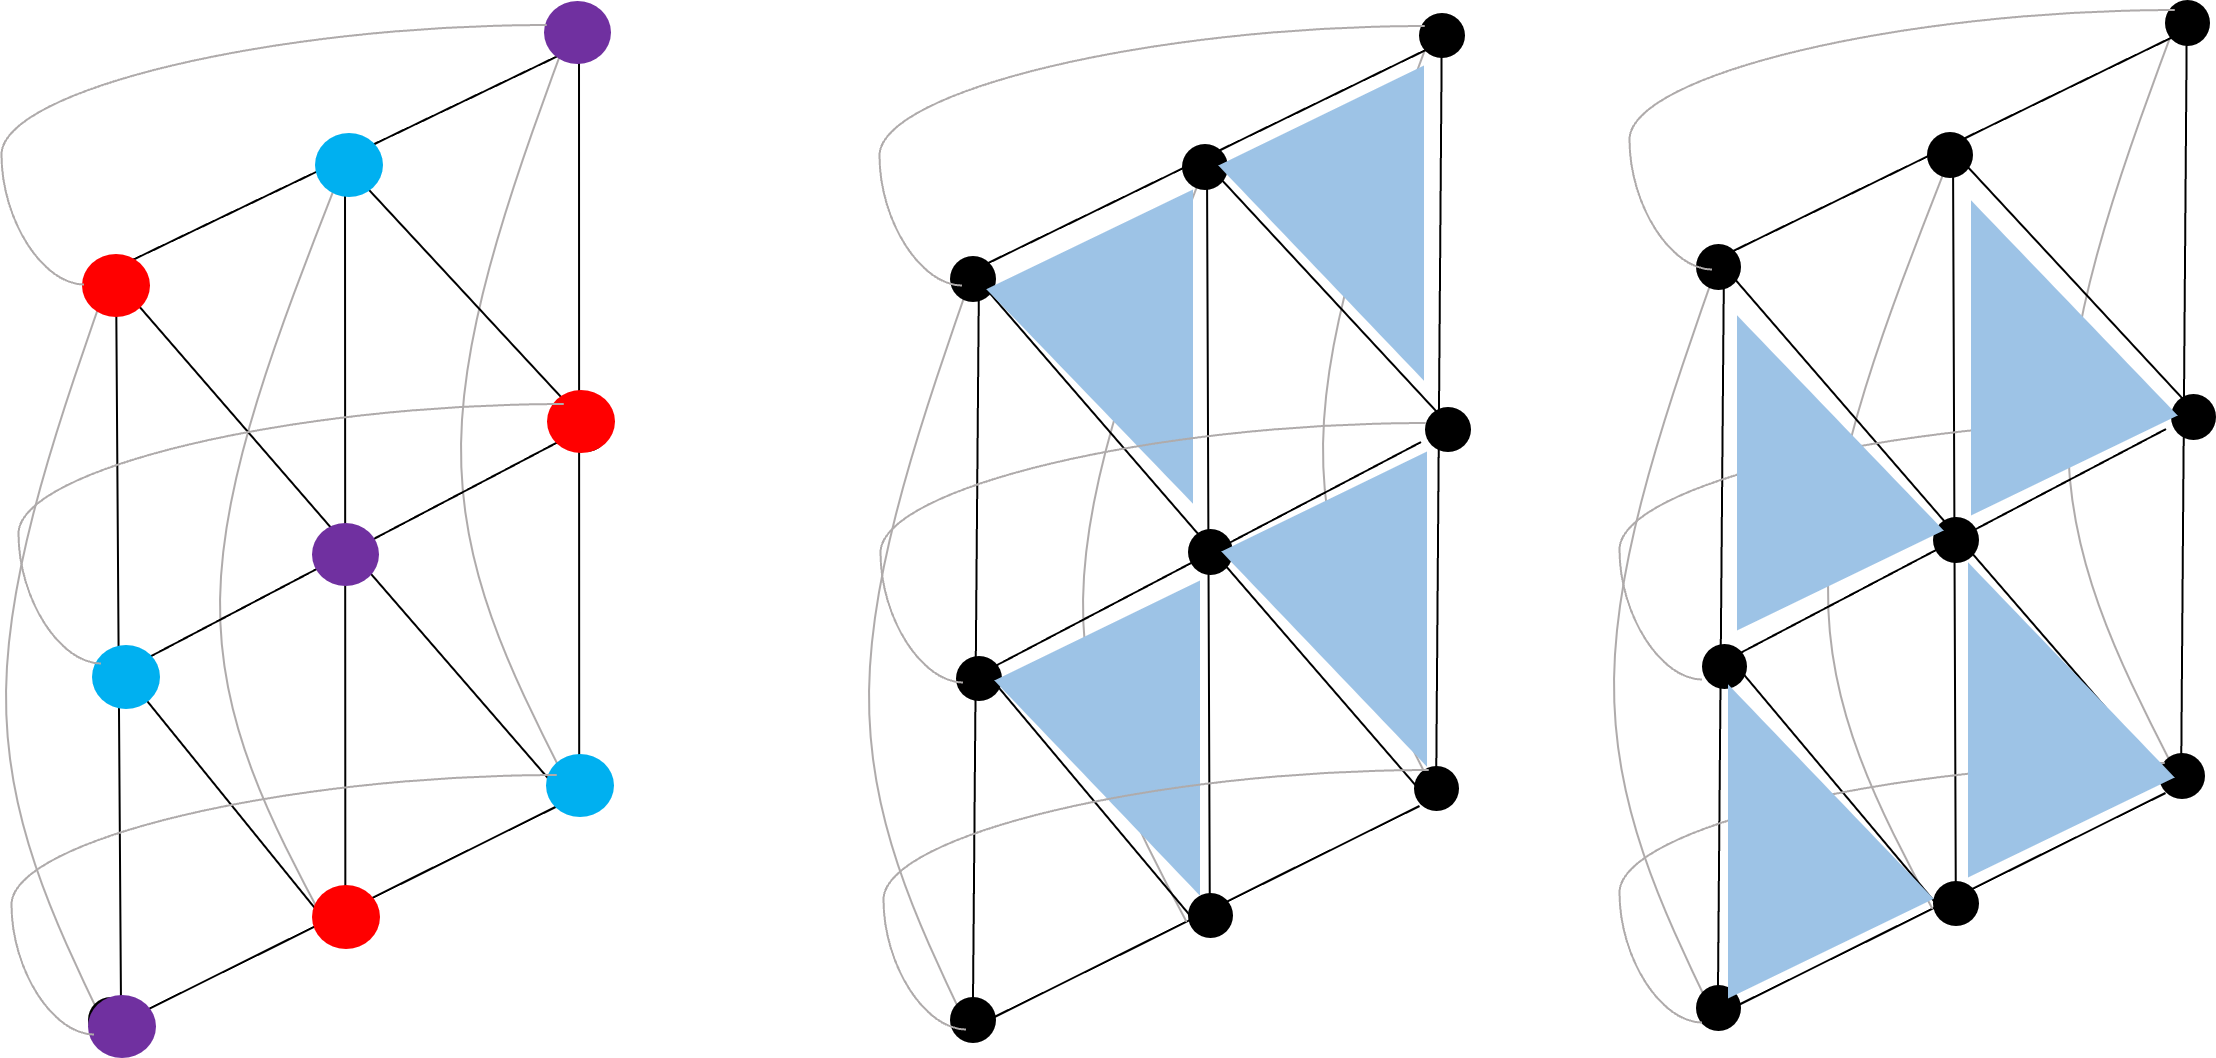
\includegraphics[width=70mm]{holyer_graph.png}
		\caption{$H_{3,3}$, 3-colouring, true triangulation, false triangulation}
\end{wrapfigure}

Consider the graph $H_{3,p}$ defined as $V=\{(x_1,x_2,x_3)\in \mathbb{Z}^3|x_1+x_2+x_3=0\text{ mod }p \}$, $(x_1,x_2,x_3)$ and $(y_1,y_2,y_3)$ are adjacent if there exists distinct $i,j,k$ such that $x_i=y_i \text{ mod }p $, $x_j=(y_j+1) \text{ mod }p $ and $x_k=(y_k-1) \text{ mod }p $.

Observe $H_{3,p}$ is a tripartite graph iff $p=0 \text{ mod }3$.

$H_{3,p}$ has only two triangulations, termed a true and a false triangulation, we say $G=T$ if graph $G$ has a true triangulation and $G=F$ if it has a false triangulation. We glue graphs together by taking a set of vertices in $G_1$ and making them the 'same' as a set of vertices in $G_2$, such that the vertices sets are the same size.

\begin{wrapfigure}{r}{5cm}
		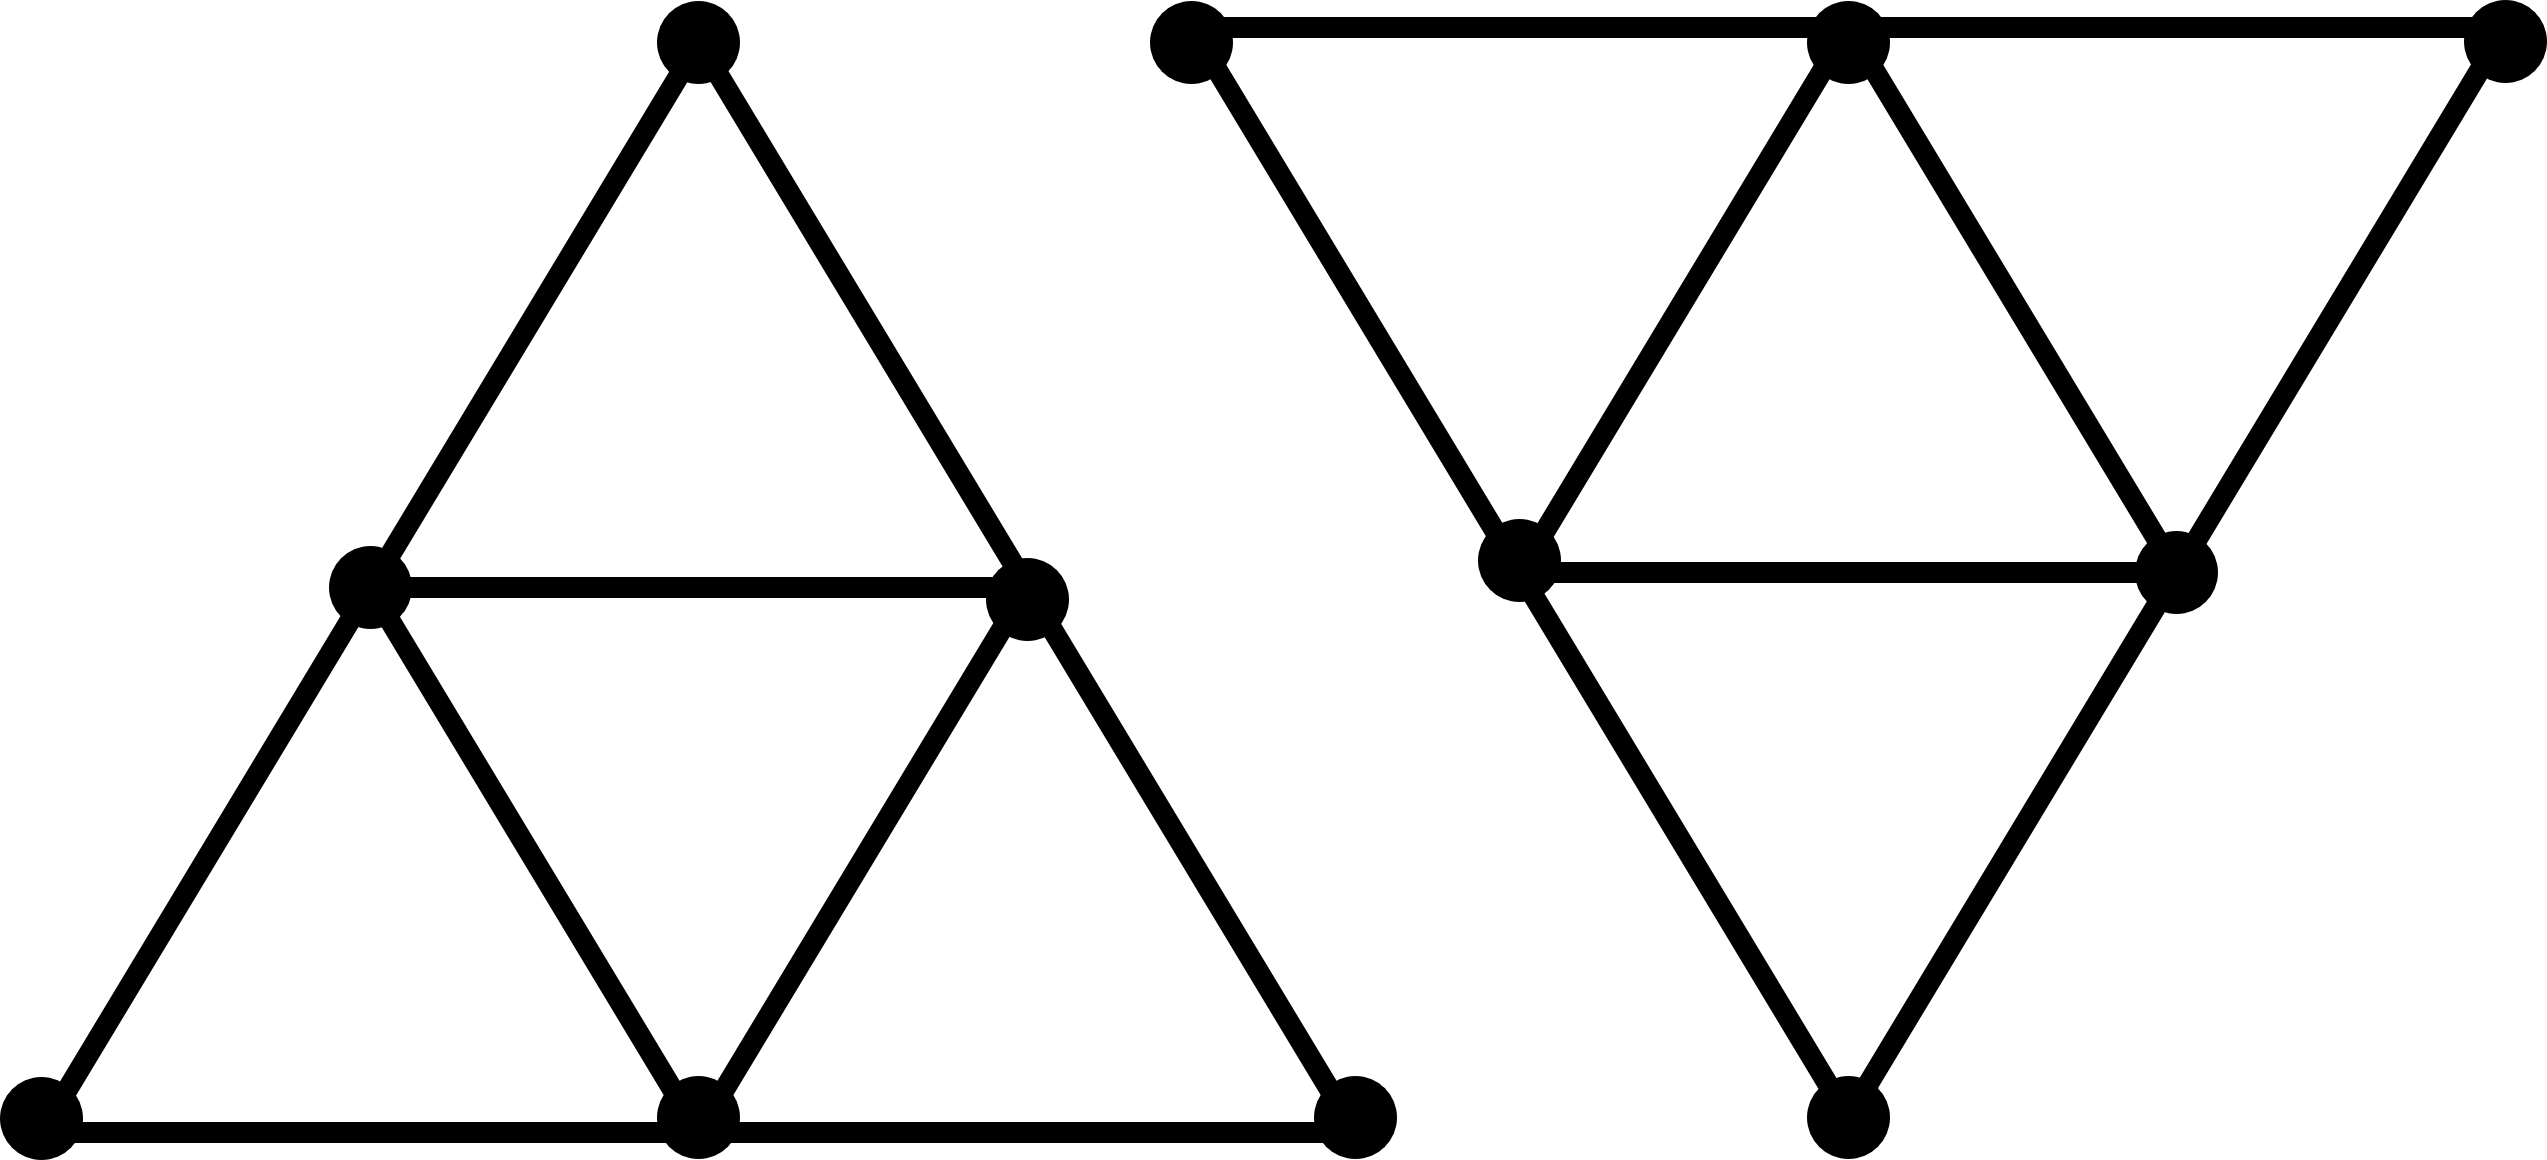
\includegraphics[width=50mm]{patches.png}
		\caption{A-patch, B-patch}
\end{wrapfigure}

\textbf{Lemma:} Connecting two $H_{3,p}$ by two A-patches then our triangulations of these graphs can be of the form $(T,T)$, $(T,F)$ or $(F,T)$

\textbf{Lemma:} Connecting two $H_{3,p}$ by two A-patches then removing the centre triangles from both graphs we get triangulations $(T,F)$ or $(F,T)$.

\textbf{Lemma:} Connecting $x$ $H_{3,p}$ by $x$ A-patches then removing the centre triangles from all graphs we get triangulations $\in \{(a_1,...,a_x)| a_i=F\text{ and } \forall j\neq i\text{ } a_j=T \}$.

Using the above lemmas we can change a 3SAT boolean expression into a tripartite graoh that has a triangulation iff the boolean expression is satisfiable.

For $b_i\in B$ create $H_{3,p}$ called $G_{b_i}$. For all $c_j\in C$, for each literal $l_{i,j}$ $i\in [1,2,3]$  create $H_{3,p}$ called $G_{i,j}$. For $b_i \in B$ connect an A-patch to each $G_{i,j}$ such that $l_{i,j}=b_i$ and a B-patch to $G_{i,j}$ such that $l_{i,j}=\neg b_i$. For each $c_i\in C$ connect an A-patch from $G_{1,i}$, $G_{2,i}$ and $G_{3,i}$ then delete the centre triangle. Select p large enough to prevent patch overlap. $G = \{G_{b_i} \forall b_i \in B\}\cup\{G_{i,j} \forall c_j\in C\text{ and }l_{i,j}\in c_j \}$

If a triangulation $T$ of $G$ exists then: 
\begin{itemize}
\item $G_{b_i}$ has a true or false triangulation. 
\item If $l_{i,j}=b_i$, $G_{i,j}= T$ when $G_{b_i}=F$ but when $G_{b_i}=T$ $G_{i,j}$ can be a true or false triangulation. 
\item If $l_{i,j}=\neg b_i$, $G_{i,j}= T$ when $G_{b_i}=T$ but when $G_{b_i}=T$ $G_{i,j}$ can be a true or false triangulation. 
\item Exactly one of $G_{i,1}, G_{i,2}$ or $G_{i,3}$ have a false triangualtion and the other have a true triangulations.
\end{itemize}

These statements come from the above lemmas and allow a 3SAT formula to be converted to the problem of triangulating a tripartite graph. Conversely if we can find a triangulation this will give us a truth assignment which can be determined from the $G_{b_i}$ portions of the graph. If $G_{b_i}$ is a true triangulation $b_i = T$ in our truth assignment. $\square$
  \end{block}


  \begin{block}{References}
    \nocite{*}
    \footnotesize{\bibliographystyle{plain}\bibliography{poster}}
  \end{block}
\end{column}

\separatorcolumn
\begin{column}{\colwidth}
 
  \begin{block}{Latin Square $\geq_p$ Triangulated Tripartite Graph}

\begin{wrapfigure}{r}{5cm}
		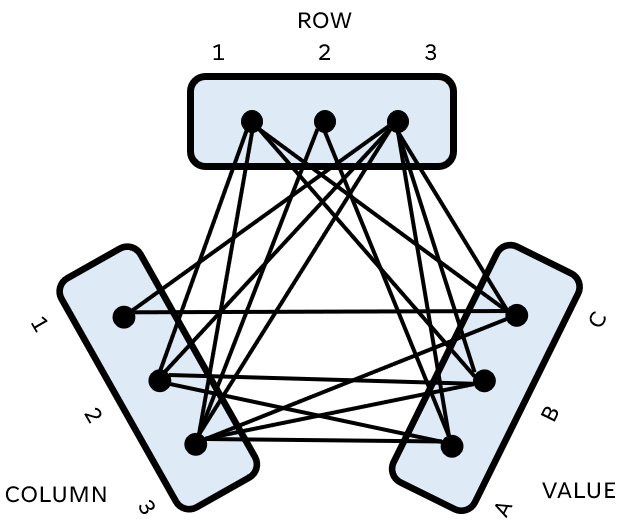
\includegraphics[width=50mm]{ttg.png}
		\caption{Tripartite Graph equivalent to partial $L$}
\end{wrapfigure}

Observe completing a partial Latin square is equivalent to triangulating tripartite graph, we map the Latin square to this through the following: 
given tripartite graph $G=(V,E)$ label vertices in $V_1$ with distinct lables $\{r_1,...r_n\}$, label vertices in $V_2$ with distinct lables $\{c_1,...c_n\}$ and label vertices in $V_3$ with distinct lables $\{e_1,...e_n\}$. Add edges such that:

\begin{itemize}
\item{If $L(i,j) = 0$ then add the edge $(r_i,c_j)$ }
\item{If for all $i \in [0,...,n]$ and constant j, $L(i,j) \neq k$ then add the edge $(r_i,e_k)$}
\item{If for all $j \in [0,...,n]$ and constant i, $L(i,j) \neq k$ then add the edge $(c_j,e_k)$}
\end{itemize}
This graph has a triangulation iff $L(i,j)$ can be solved.

Let us show every uniform tripartite graph is the above formulation of a Latin square.

\textbf{Def$^{\text{n}}$:} A Latin framework $LF$ for tripartite graph $G$, size $(r,s,t)$ is a $r \times s$ array with values $[1,...,t]$. With constraints:
\begin{itemize}
\item{Each row/column contain each element only once.}
\item{If $(r_i,c_j)\in E$ then $LF(i,j)=$empty else $LF(i,j)= k$ $k\in [1,...,t]$}
\item{If $(r_i,e_k)\in E$  then for constant i $LF(i,j)\neq k$}
\item{If $(c_i,e_k)\in E$  then for constant j $LF(i,j)\neq k$}
\end{itemize}
If $r=s=t$ then $LF$ is a latin square which can be completed iff $G$ has a triangle partition.

\textbf{Lemma:} For graph $G=(V,E)$ with $|V|=n$, there's a Latin framework of size $(n,n,2n)$.

Define $LF$ an $n \times n$ array. For $(r_i,c_j)\in E$ $LF(i,j)=0$ else $LF(i,j)=1+n+((i+j)\text{mod }n)$.$ LF$ is a latin framework. 

\textbf{Lemma:} Latin framework $L$  $(r,s,t)$ for uniform tripartite graph $G$. $R(k) =$ the number of times $k$ appears in $L$ plus half $|e_k|$. Whenever $R(k)\ge r+s-t$ for $1 \le k \le t$, L can be extended to $(r,s+1,t)$ to give $L'$ in which $R'(k)\ge r + s+1-t$ for all $1\le k \le t$.

\textbf{Lemma:} Latin framework of size $(r,s,s)$ can be extended to a Latin framework size $(s,s,s)$.

Given a tripartite graph $G$, if it is not uniform then no triangulation exists, else we apply above to produce a latin framework of size $(2n,2n,2n)$ in polynomial time. This is a Latin square which can be completed iff G has a triangulation. The latin square problem has been reduced to the triangulating a tripartite graph problem. $\square$

  \end{block}
\begin{block}{Sudoku $\geq_p$ Latin Square}

\textbf{Lemma:} Let $S$ be a Sudoku problem with the following construction 
\begin{equation}
	S(i,j) =\begin{cases}
0 \qquad\qquad\qquad\qquad\qquad\qquad\text{when } (i,j) \in S_l \\ 
((i-1 \text{ mod } n)n + \left\lfloor{i-1/n}\right\rfloor+j-1)\text{ mod } n^2 +1 \quad\text{otherwise}
\end{cases}
\end{equation}
where $S_l=\{(i,j)| \left\lfloor{i-1/n}\right\rfloor=0 \text{ and }(j \text{ mod }n)=1\}$. Then there exists an augmentation $S'$ to complete the sudoku puzzle if and only if the square $L$ such that $L(i,j/n)=(S'(i,j)-1)/n+1$ for all $(i,j) \in S_l$ is a Latin square.

\begin{wrapfigure}{l}{12.8cm}
\begin{tikzpicture}[scale=.5]
\begin{scope}[xshift=4cm]
    \draw (0, 0) grid (3, 3);
    \setcounter{rowa}{1}
    \setrowa {1}{}{}
    \setrowa {2}{3}{} 
    \setrowa {}{}{} 
    \node[anchor=center] at (1.5, -0.5) {$L$};
  \end{scope}
  \begin{scope}[xshift=8cm]
    \draw (0, 0) grid (9, 9);
    \draw[very thick, scale=3] (0, 0) grid (3, 3);
    \setcounter{row}{1}
    \setrow {0}{2}{3}  {0}{5}{6}  {0}{8}{9}
    \setrow {0}{5}{6}  {0}{8}{9}  {0}{2}{3}
    \setrow {0}{8}{9}  {0}{2}{3}  {0}{5}{6}
    \setrow {2}{3}{4}  {5}{6}{7}  {8}{9}{1}
    \setrow {5}{6}{7}  {8}{9}{1}  {2}{3}{4}
    \setrow {8}{9}{1}  {2}{3}{4}  {5}{6}{7}
    \setrow {3}{4}{5}  {6}{7}{8}  {9}{1}{2}
    \setrow {6}{7}{8}  {9}{1}{2}  {3}{4}{5}
    \setrow {9}{1}{2}  {3}{4}{5}  {6}{7}{8}
    \node[anchor=center] at (4.5, -0.5) {Lemma construction of $S$};
  \end{scope}
  \begin{scope}[xshift=18.5cm]
    \draw (0, 0) grid (9, 9);
    \draw[very thick, scale=3] (0, 0) grid (3, 3);
    \setcounter{row}{1}
    \setrow {1}{2}{3}  {0}{5}{6}  {0}{8}{9}
    \setrow {4}{5}{6}  {7}{8}{9}  {0}{2}{3}
    \setrow {0}{8}{9}  {0}{2}{3}  {0}{5}{6}
    \setrow {2}{3}{4}  {5}{6}{7}  {8}{9}{1}
    \setrow {5}{6}{7}  {8}{9}{1}  {2}{3}{4}
    \setrow {8}{9}{1}  {2}{3}{4}  {5}{6}{7}
    \setrow {3}{4}{5}  {6}{7}{8}  {9}{1}{2}
    \setrow {6}{7}{8}  {9}{1}{2}  {3}{4}{5}
    \setrow {9}{1}{2}  {3}{4}{5}  {6}{7}{8}
    \node[anchor=center] at (4.5, -0.5) {$S$ augmented};
  \end{scope}
\end{tikzpicture}
\end{wrapfigure}

Given partial Latin Square $L$, construct $S$ as above and augment so $\forall (i,j)$ such that $L(i,j)\neq0$ $S(i,n(j-1)+1)= n(L(i,j)-1)+1$. $S$ after the augmentation can be solved if and only if $L$ can be solved. $\square$

  \end{block}
\end{column}

\separatorcolumn

\end{columns}
\end{frame}

\end{document}